\documentclass[12pt,italian]{report}
\usepackage{tesi}

%
%			INFORMAZIONI SULLA TESI
%			DA COMPILARE!
%

% CORSO DI LAUREA:
\def\myCDL{Corso di Laurea triennale in\\Informatica}

% TITOLO TESI:
\def\myTitle{ANALISI DEI DATI PER PROBLEMI DI\\ MEDICINA LEGALE}

% AUTORE:
\def\myName{Alessandro Beranti}
\def\myMat{Matr. Nr. 855489}

% RELATORE E CORRELATORE:
\def\myRefereeA{Prof. Dario Malchiodi}
\def\myRefereeB{Prof. Anna Maria Zanaboni}

% ANNO ACCADEMICO
\def\myYY{2018-2019}

% Il seguente comando introduce un elenco delle figure dopo l'indice (facoltativo)
%\figurespagetrue

% Il seguente comando introduce un elenco delle tabelle dopo l'indice (facoltativo)
%\tablespagetrue

%
%			PREAMBOLO
%			Inserire qui eventuali package da includere o definizioni di comandi personalizzati
%

% Package di formato
\usepackage[a4paper]{geometry}		% Formato del foglio
\usepackage[italian]{babel}			% Supporto per l'italiano
\usepackage[utf8]{inputenc}			% Supporto per UTF-8
%\usepackage[a-1b]{pdfx}			% File conforme allo standard PDF-A (obbligatorio per la consegna)

% Package per la grafica
\usepackage{graphicx}				% Funzioni avanzate per le immagini
\usepackage{hologo}					% Bibtex logo with \hologo{BibTeX}
%\usepackage{epsfig}				% Permette immagini in EPS
%\usepackage{xcolor}				% Gestione avanzata dei colori

% Package tipografici
\usepackage{amssymb,amsmath,amsthm} % Simboli matematici
\usepackage{listings}				% Scrittura di codice

% Package ipertesto
\usepackage{url}					% Visualizza e rendere interattii gli URL
\usepackage{hyperref}				% Rende interattivi i collegamenti interni
\usepackage{caption}
\usepackage{booktabs}
\usepackage{verbatim}
\usepackage{adjustbox}
\usepackage{makecell}
\usepackage{xcolor,colortbl}
\lstset{language=Python} 
\setcounter{tocdepth}{4}
\setcounter{secnumdepth}{4}

\begin{document}

% Creazione automatica del frontespizio
\frontespizio
\beforepreface

% 
%			PAGINA DI DEDICA E/O CITAZIONE
%			facoltativa, questa è l'unica cosa che dovete formattare a mano, un po' come vi pare
%

{\raggedleft \large \sl Questo lavoro \`{e} dedicato a tutti gli studenti\\
	
	\vspace{2cm}
	
	``Io studio,\\ma studiate pure voi,\\che se studio solo io non serve a un c\dots o''
	
	\bigskip
	
	\--- Gli scarabocchi di Maicol \& Mirco\\
  
	\vspace{2cm}
	
	``No tale is so good \\ that it can't be spoiled \\ in the telling''
	
	\bigskip
	
	\--- Proverbio\\}
         
% 
%			PREFAZIONE (facoltativa)
%

%\prefacesection{Prefazione}
%Le prefazioni non sono molto comuni, tuttavia a volte capita che qualcuno voglia dire qualcosa che esuli dal lavoro in s\'e (come un meta-commento sull'elaborato), o voglia fornire informazioni riguardanti l'eventuale progetto entro cui la tesi si colloca (in questo caso \`e probabile che sia il relatore a scrivere questa parte).

%
%			RINGRAZIAMENTI (facoltativi)
%

\prefacesection{Ringraziamenti}
Questa sezione, facoltativa, contiene i ringraziamenti.

%
%			Creazione automatica dell'indice
%

\afterpreface

% 
%			CAPITOLO 1: Introduzione o Abstract
% 

\chapter*{Introduzione}
\label{cap:introduzione}

Questo documento ha una duplice funzione: da un lato mostra un esempio completo di elaborato finale redatto in \LaTeX\ e conforme allo standard PDF/A, e dall'altro contiene suggerimenti e risposte a domande frequenti poste dagli studenti. Se ne raccomanda, pertanto, un'attenta lettura.

\chapter{Machine Learning}
Il termine Machine Learning, o apprendimento automatico in italiano, si riferisce alla capacità dei computer di apprendere e agire senza essere programmati esplicitamente.
Gli strumenti di machine learning si occupano di dotare i programmi della capacità di ``apprendere'' e adattarsi agli input forniti.
Al giorno d'oggi siamo circondati da tecnologie basate sull'apprendimento automatico:
\begin{itemize}
	\item software che rilevano lo spam a partire dai nostri messaggi e-mail, 
	\item motori di ricerca che imparano a ordinare i risultati di una query di ricerca al fine di mostrare prima quelli più rilevanti, 
	\item transazioni con carta di credito protette da un software che impara a rilevare le frodi, 
	\item fotocamere digitali che imparano a rilevare i volti, 
	\item assistenti digitali che imparano a riconoscere i comandi vocali, 
	\item veicoli autonomi addestrati a guidare senza intervento umano, 
	\item applicazioni scientifiche come la bioinformatica, la medicina e l'astronomia.
\end{itemize}
\section{Come funziona il Machine Learning}
\label{ComefunzionailMachineLearning}
Nel Machine Learning vengono usati metodi statistici che applicano un procedimento di induzione a partire da dati che rappresentano istanze di un problema, accoppiate con una possibile soluzione, per migliorare le prestazioni di algoritmi o fare previsioni più accurate.
La qualità e la dimensione dei dataset (collezione di dati), raccolti o resi disponibili e utilizzati nel processo sono fondamentali per il successo e l'accuratezza delle previsioni fatte.

Il processo parte da un domain set $X$, ovvero una raccolta arbitraria di dati, che rappresentano gli oggetti che si desidera etichettare. Essi possono essere già etichettati nel caso di apprendimento supervisionato come non esserlo nel caso non supervisionato. Questo set di dati rappresenta l'input dell'algoritmo di apprendimento che si è scelto di usare. Il risultato è un modello a cui è associato un errore di generalizzazione, ovvero la probabilità che non venga predetta l'etichetta corretta.
Il domain set può essere diviso in due sottoinsiemi: il \textit{training set}, insieme di dati che vengono scelti per compiere l'addestramento, e il \textit{test set} che viene utilizzato per valutare le prestazioni del modello predittivo.

Una categorizzazione dei compiti del machine learning si ha quando si considera l'output desiderato del sistema che può essere di diversi tipi:
\begin{itemize}
	\item classificazione, significa che il dato è categorico \cite{SupervisedMachineLearning} e viene fatta una divisione dei dati in classi o etichette. Può essere una classificazione binaria, nel quale le etichette sono soltanto due, oppure multiclasse, etichette sono tre o più,
	\item regressione, usata per predire un valore assimilabile a una quantità che varia in un insieme continuo, per esempio il prezzo di una casa date la dimensione e la metratura \cite{SupervisedMachineLearning},
	\item clustering, in cui un insieme di input viene diviso in gruppi in modo che i singoli elementi siano simili agli altri punti dello stesso insieme e diversi dagli elementi degli altri; diversamente da quanto accade per la classificazione, i gruppi non sono noti prima, rendendolo tipicamente un compito non supervisionato \cite{Introductiontodatamining}.
\end{itemize}
Gli algoritmi di apprendimento automatico vengono tipicamente organizzati in quattro categorie, a seconda della natura del ``segnale'' utilizzato per l'apprendimento o del ``feedback'' disponibile al sistema di apprendimento. Queste categorie, anche dette paradigmi, sono:
\begin{itemize}
	\item Machine Learning supervisionato,
	\item Machine Learning non supervisionato,
	\item Machine Learning per rinforzo,
	\item Machine Learning semi-supervisionato.
	
\end{itemize}

\subsection{Apprendimento supervisionato}
\label{apprendimentoSupervisionato}
Attraverso l’apprendimento supervisionato si cerca di costruire un modello partendo da dati di addestramento etichettati, a partire dai quali si tenta di fare previsioni su dati non disponibili o futuri. Con il termine ``supervisione'' si intende quindi che nell'insieme dei campioni (o dataset), i segnali di output desiderati sono già noti poiché precedentemente etichettati.
Nell'apprendimento supervisionato l'output può essere sia numerico che categorico, quindi può trattarsi rispettivamente di regressione e classificazione; siccome il tirocinio ha riguardato solo quest'ultima d'ora in avanti parleremo di classificazione.

Esistono molti algoritmi per svolgere apprendimento supervisionato, durante il tirocinio ho avuto modo di usare:
\begin{itemize}
	\item Support Vector Machine,
	\item Decison Tree Classifier,
	\item Random Forest Classifier,
	\item Gaussian Naive Bayes,
	\item Linear Discriminant Analysis,
	\item Reti Neurali Multi-Strato.
\end{itemize}

\subsubsection{Support Vector Machine}
\label{sec:SVC}
Il Support Vector Machine (SVM) è un algoritmo di apprendimento automatico supervisionato che può essere usato sia per scopi di classificazione che di regressione, si può applicare sia a problemi binari, sia a problemi multiclasse. Nel paragrafo seguente verrà descritto solo la versione per la classificazione binaria poichè è quella che ho usato durante il tirocinio.

L'SVM è basato sull'idea di riuscire a trovare un iperpiano che divida al meglio un set di elementi in due classi distinte \cite{LectureNotesNg}. Definiamo alcuni elementi che ci serviranno successivamente.

\begin{figure}[h]
	\centering
	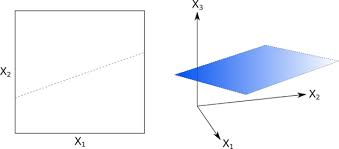
\includegraphics[width = 80mm]{immagini/2e3dimensionisvc}
	\caption{A sinistra grafico bidimensionale e destra tridimensionale}
\end{figure}

\begin{itemize}
	\item Iperpiano: nel caso in cui si abbiano solo due dimensioni spaziali nel qualche si trovano le descrizioni degli oggetti da classificare $x_1$ e $x_2$, l'iperpiano è raffigurato come una linea che separa un insieme di dati \cite{LectureNotesNg}. Nel caso in cui le dimensioni siano 3, l'iperpiano è raffigurato come un piano, ( cfr. Figura 1).
	Con più di 3 dimensioni viene definito ``iperpiano''.
	\item Support Vector: chiamati vettori di supporto in italiano, sono i punti che si trovano piu vicini all'iperpiano che divide i dati.
	\item Margine: è la distanza tra i vettori di supporto di due classi diverse. A metà di questa distanza viene tracciato l'iperpiano, (cfr. Figura 2).
\end{itemize}

\begin{figure}[h]
	\centering
	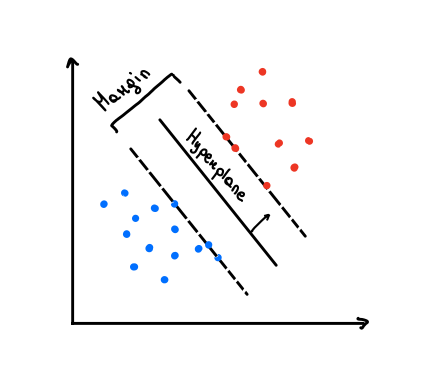
\includegraphics[width = 70mm]{immagini/marginEhiperplane}
	\caption{Iperpiano e margine}
\end{figure}

Il Support Vector Machine ha l'obiettivo di identificare l'iperpiano che divide meglio i vettori di supporto in classi. Esistono due algoritmi diversi a seconda se esista o meno l'iperpiano.

\begin{itemize}
	\item Nel caso in cui esista e in particolare ce ne sia più di uno cerca quello con il margine più alto tra i vettori di supporto in modo da evidenziare meglio la divisione tra i dati. La massimizzazione del margine porta ad avere degli iperpiani che tendono a minimizzare le probabilità di errore quando classificano nuovi dati. 
	\item Se l'iperpiano cercato non esiste, Support Vector Machine usa una mappatura non lineare per trasformare i dati di training $X$, in uno spazio di dimensione superiore rispetto a quello dei dati originali in modo che le immagini dei dati di due classi siano separati da un iperpiano, che sarà scelto per la suddivisione dei dati. 
\end{itemize}

In dati linearmente separabili è possibile individuare un iperpiano in cui si possono distinguere due semispazi. Nella figura 3 è visibile come sia possibile disegnare un numero infinito di linee rette per separare i diversi elementi. Il problema è trovare quale tra le infinite rette risulti ottimale, ossia quella che, a fronte di una generica nuova osservazione, classifichi nel modo corretto l'osservazione.

\begin{figure}[h]
	\centering
	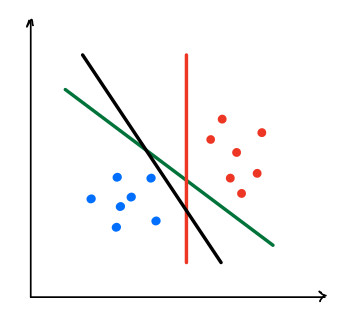
\includegraphics[width = 60mm]{immagini/linearmente-separabili}
	\caption{Infinite rette possono separare gli elementi}
\end{figure}

Dato un training set etichettato:

\begin{center}
	\[
	\ (x_1, y_1), ..., (x_n, y_n)
	\ \forall i 
	\ x_i \in R^{d},
	\ y_i \in  \{ -1, +1 \}
	\]
\end{center}
dove $x_i$ sono i punti da classificare e $y_i$ sono le etichette.

Un iperpiano è definito come 
\begin{center}
	\[w_0 + w_1z_1 + w_2z_2 +...+ w_mz_m= 0,\]
\end{center}
dove $\omega$ è il vettore di peso, $z$ è il vettore di caratteristiche di input e $w_0$ è il bias.
In sostanza in $m$ dimensioni un iperpiano di separazione è una combinazione lineare di tutte le dimensioni uguagliate a 0.
Ragionando a due dimensioni per semplificare il problema abbiamo che 
\begin{center}
	\[w_0 + w_1z_1 + w_2z_2 = 0.\]
\end{center}
I punti che stanno sopra l'iperpiano e che rappresentano un classe soddisfano la seguente condizione:
\begin{center}
	\[w_0 + w_1z_1+w_2z_2 > 0,\]
\end{center}
mentre qualsiasi punto che si trova sotto l'iperpiano, appartiene all'altra classe, che è soddisfatta dalla seguente condizione :
\begin{center}
	\[w_0 + w_1z_1+w_2z_2 < 0,\]
\end{center}
L'algoritmo di apprendimento per SVM, in realtà, riscrive queste condizioni in modo più stringente:
\begin{center}
	\[w_0 + w_1z_{i,1}+w_2z_{i,2} \geq 1,
	\ \forall i 
	\ t.c. 
	\ y_i=1,\]
	\[
	\ w_0 + w_1z_{i,1}+w_2z_{i,2} \leq -1 
	\ \forall i 
	\ t.c.
	\ y_i = -1,\]
\end{center}
dove $z_{i,1}$ rappresenta la prima componente dell'i-vettore e $z_{i,2}$ la seconda componente dell'i-esimo vettore.

Se il vettore dei pesi è indicato da $w$ e $\parallel w \parallel$ è la sua norma, allora la dimensione del margine massimo è 
\begin{center}
	\[ \frac{1}{\left || w \right ||} + \frac{1}{\left || w \right ||} = \frac{2}{\left || w \right ||},\]
\end{center}
ciò significa che minimizzando la norma del vettore peso $w$, avremo margine massimo che determina l'iperpiano ottimale.

Non è però sempre possibile dividere i dati tramite un iperpiano, come esemplificato in Figura 4.

\begin{figure}[h]
	\centering
	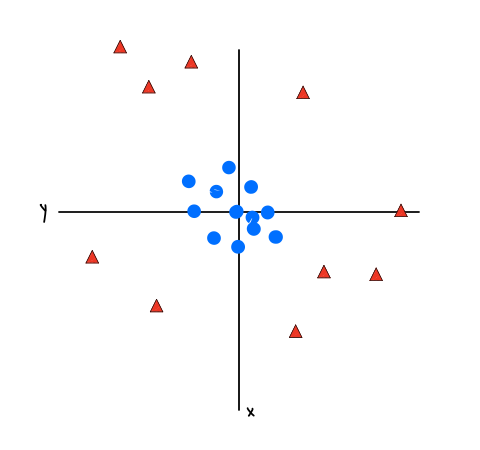
\includegraphics[width = 70mm]{immagini/nonLineare}
	\caption{Non sempre è possibile dividere i dati linearmente}
\end{figure}

Per utilizzare la classificazione tramite iperpiani anche per dati che avrebbero bisogno di funzioni non lineari per essere separati, è necessario ricorrere alla tecnica degli spazi immagine ($feature$ $spaces$). Questo metodo, che sta alla base della teoria delle SVM, consiste nel mappare i dati iniziali in uno spazio di dimensione superiore.  Presupponendo quindi $m > n$, per la mappa si utilizza una funzione
\begin{equation}
	\phi: \mathbb{R}^{n} \rightarrow \mathbb{R}^{m},
\end{equation}
attraverso la funzione $\phi$ i dati vengono mappati in uno spazio a più dimensioni, ciò comporta che i dati potrebbero essere linearmente separabili e quindi sarebbe possibile trovare un iperpiano che li separi \cite{LectureNotesNg}.

La tecnica degli spazi immagine è particolarmente interessante per algoritmi che utilizzano i dati di training $x_i$ solo attraverso prodotti scalari $x_i \cdot x_j$. In questo caso nello spazio $\mathbb{R}^{m}$ non si devono trovare esplicitamente $\phi(x_i)$ e $\phi (x_j)$ ma basta calcolare il loro prodotto scalare $\phi (x_i) \cdot \phi (x_j)$. Per rendere semplice questo ultimo calcolo, che in spazi di dimensioni elevate diventa molto complicato, si utilizza una funzione detta \textit{kernel} che restituisce direttamente il prodotto scalare delle immagini:
\begin{equation}
K(x_i, x_j) = \phi (x_i) \cdot \phi (x_j),
\end{equation}
Esistono svariati \textit{kernel}, i più utilizzati sono:
\begin{itemize}
	\item il kernel lineare: $K(x, y) = x \cdot y$,
	\item il kernel polinomiale: $K(x, y) = (x \cdot y)^{d}$ oppure $K(x, y) = (1 + x \cdot y)^{d}$,
	\item il kernel gaussiano: $K(x,y) = \exp (- \left || x-y \right || ^2)/(2 \sigma 2)$,
	\item il kernel sigmoide: $K(x,y) = \tanh(k x \cdot y - \delta)$.
\end{itemize}

\subsubsection{Decision Tree Classifier}
Il Decision Tree Classifier è un metodo di apprendimento supervisionato usato sia per scopi di classificazione che di regressione. Utilizza un albero decisionale, \textit{decision tree}, composto da \cite{DataMiningandKnowledgeDiscoveryHandbook}:
\begin{itemize}
	\item nodi non terminali: rappresentano un test su uno o più caratteristiche,
	\item ramo: rappresenta un esito del test,
	\item foglia: rappresenta una possibile classe.
\end{itemize}

Dato un insieme di dati è possibile costruire un numero esponenziale di alberi di decisione. Alcuni alberi sono più efficienti di altri ma trovare l'albero ottimo è una cosa computazionalmente infattibile a causa dello spazio esponenziale nel quale bisogna cercare. Tuttavia esistono algoritmi che riescono, in un tempo ragionevole, a trovare un albero efficiente anche se non corrisponde all'ottimo. Questi algoritmi spesso implementano una strategia greedy che crea l'albero facendo una serie di decisioni localmente ottime su quale caratteristica dei dati usare per partizionare i dati \cite{Introductiontodatamining}.
Uno di questi algoritmi è l'algoritmo di Hunt nel quale l'albero di decisione viene costruito ricorsivamente partizionando il training set in sottoinsiemi sempre più piccoli. Sia $D_t$ l'insieme dei dati di training che sono associati al nodo $t$ e sia $y = {y_1, y_2,...,y_c}$ le etichette. La definizione ricorsiva dell'algoritmo di Hunt è la seguente \cite{Introductiontodatamining}.
\begin{itemize}
	\item se tutti i dati in $D_t$ appartengono alla stessa classe $y_t$, allora $t$ è una foglia etichettata come $y_t$
	\item se $D_t$ contiene dati che appartengono a più di una classe, viene selezionata una caratteristica per eseguire un test per partizionare i dati in sottoinsiemi più piccoli. Viene creato un nodo figlio per ogni risultato della condizione del test e i dati in $D_t$ vengono divisi in base al risultato del test. L'algoritmo viene applicato in modo ricorsivo ad ogni nodo figlio.
\end{itemize}

La misura di selezione degli attributi è un'euristica per selezionare il criterio di suddivisione che divide i dati in modo da massimizzare l'omogeneità dei sottoinsiemi di dati. I più famosi sono l'entropia e l'indice di Gini \cite{DataMiningandKnowledgeDiscoveryHandbook}.

\subsubsection{Random Forest Classifier}
Il Random Forest Classifier è un algoritmo di apprendimento supervisionato. Esso considera più alberi di decisione che operano come un insieme. Ogni albero della foresta genera una previsione e quella che compare più frequentemente diventa la previsione del modello \cite{RandomForest}.

\begin{figure}
	\centering
	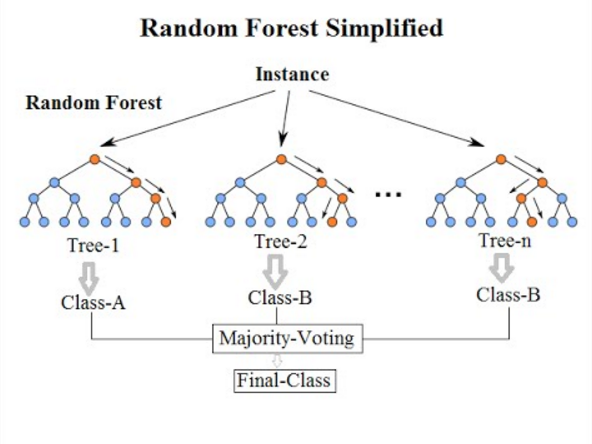
\includegraphics[width = 100mm]{immagini/randomForest}
	\caption{Random Forest composto da più alberi di decisione}
\end{figure}

Il concetto fondamentale dietro una foresta casuale risiede nel fatto che un grande numero di alberi non correlati tra loro che operano insieme tendono a essere più efficienti di un singolo albero.

La bassa correlazione è la chiave, modelli non correlati possono produrre previsioni d'insieme più accurate di qualsiasi singola previsione. La ragione risiede nel fatto che, anche se alcuni alberi potrebbero sbagliare, molti altri avranno ottenuto la previsione corretta.
\subsubsection{Gaussian Naive Bayes}
Il Gaussian Naive Bayes è uno dei più semplici algoritmi di apprendimento supervisionato, e si basa sul teorema di Bayes. L'algoritmo assume che l'effetto di una particolare caratteristica in una classe sia indipendente dalle altre caratteristiche. Anche se le caratteristiche sono interdipendenti, esse vengono comunque considerate in modo indipendente\cite{Mitchell97}. Questa ipotesi, a cui ci si riferisce come indipendenza condizionale di classe, semplifica il calcolo.
Applicando il teorema di Bayes si ha
\begin{equation}
P(y | X) = \frac{P(X | y) P(y)}{P(X)},
\end{equation}
dove $y$ è un'etichetta e $X = (z_1, z_2, z_3,...,z_n)$ è il corrispondente vettore di caratteristiche.

Siccome abbiamo assunto che le caratteristiche siano indipendenti possiamo dire che:
\begin{equation}
P(y| z_1,..., z_n) = \frac{P(z_1|y) P(z_2|y)...P(z_n|y)P(y)}{P(z_1)P(z_2)...P(z_n)}.
\end{equation}
Poiché il denominatore rimane costante per un determinato input possiamo rimuoverlo e scrivere:
\begin{equation}
P(y| z_1,..., z_n) \propto P(y) \prod_{i=1}^{n} P(z_i|y).
\end{equation}
Ora dobbiamo creare un modello per classificare. Lo facciamo trovando la probabilità di un dato insieme di input per tutti i possibili valori di $y$ e prendendo l'output con la massima probabilità:
\begin{equation}
y = \arg\max P(y) \prod_{i=1}^{n} P(z_i|y).
\end{equation}
Rimane solo da calcolare $P(y)$ e $P(z_i|y)$, che sono ricavabili dal dataset dato in input al sistema.

Nel Gaussian Naive Bayes si presume che i valori continui associati a ciascuna caratteristica siano distribuiti secondo un modello gaussiano. 

Sulla base di questa assunzione è quindi possibile scrivere le probabilità condizionate che compaiono in (6) nel modo seguente
\begin{equation}
P(z_i|y) = \frac{1}{\sqrt{2\pi \sigma_y^2}} e^{-\frac{(z_i-\mu_y)^2}{2\sigma_y^2}},
\end{equation}
dove $\mu_y$ è la media e $\sigma_y$ la deviazione standard.
\subsubsection{Linear Discriminat Analysis}
Il Linear Discriminat Analysis è un algoritmo di apprendimento supervisionato il cui scopo è quello di trovare una combinazione lineare di caratteristiche che caratterizza o separa due o più classi di oggetti. La combinazione risultante può essere utilizzata come classificatore o anche per la riduzione della dimensionalità. \ref{sec:riduzione}

Il processo prevede di proiettare i dati in input su un sottospazio lineare dalle direzioni che massimizzano la divisione tra le classi. La dimensione dell'output è necessariamente inferiore al numero di classi, quindi questa è, in generale, una riduzione della dimensionalità piuttosto forte, e ha senso solo in un ambiente multiclasse.

\subsubsection{Reti Neurali Multi-Strato}
\label{MLP}
Le reti neurali multi-strato sono un modello che utilizza l'algoritmo ``backpropagation'', basato sulla minimizzazione dell'errore, per compiere apprendimento supervisionato. L'idea di base è quella del neurone umano e della rete di neuroni che compone il nostro cervello. Il componente principale di una rete neurale è detto neurone o percettrone. Esso è identificato da $n$ pesi reali $w_1, w_2,...,w_n$ e quando riceve una serie di input $x_1,x_2,...,x_n$ li moltiplica per i pesi corrispondenti, viene così prodotto un valore $v$ sommando i prodotti ottenuti a cui viene sommato un termine di bias \cite{multilayerPerceptron}.  L'output della rete è ottenuto calcolando una particolare funzione, detta funzione di attivazione, usando $v$ come argomento.

\begin{figure}[h]
	\centering
	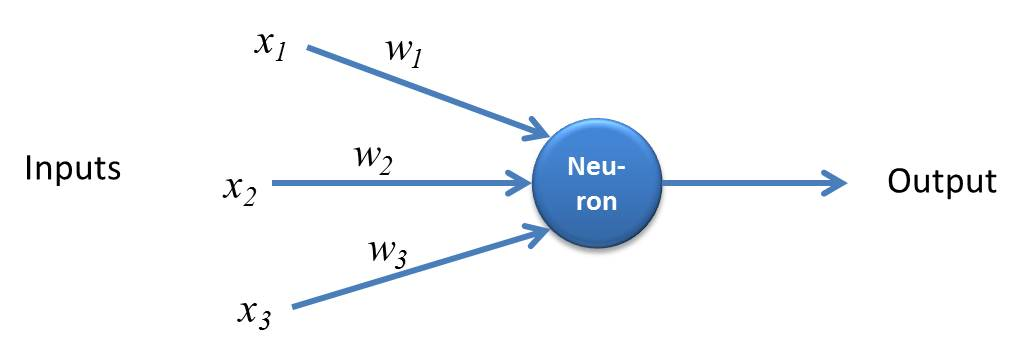
\includegraphics[width = \textwidth]{immagini/Perceptron}
	\caption{Visualizzazione di un percettrone}
\end{figure}


Una rete con un solo percettrone è chiamata a singolo livello. Esistono poi le reti multistrato, sono reti i cui percettroni sono disposti su più livelli, come indicato in Fgigura 8. Esistono tre tipi di livelli: 
\begin{itemize}
	\item livello input: costituito da un insieme di neuroni che rappresentano le caratteristiche in input,
	\item livello output: riceve i valori dall'ultimo livello hidden presente e li trasforma in valori di output, 
	\item livello hidden: livelli intermedi tra input e output, 
\end{itemize}


In questa rete ogni nodo, esclusi quelli di input, usa una funzione di attivazione non lineare per modellare il comportamento.

\begin{figure}[h]
	\centering
	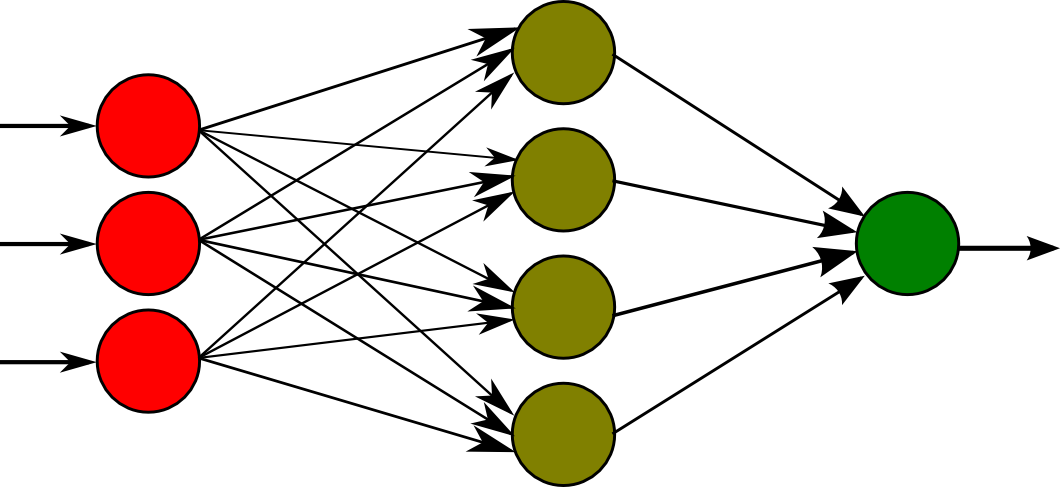
\includegraphics[width = 80mm]{immagini/Multilayer-Perceptron}
	\caption{Visualizzazione di una rete multistrato; in rosso il livello di input, al centro il livello hidden, in verde a destra il livello di output}
\end{figure}
Esistono diverse funzioni di attivazione:
\begin{itemize}
	\item Identity: $f(x) = x$,
	\item Logistic: $f(x) = \frac{1}{1 + e^{-x}}$,
	\item Tanh: $f(x) = \tanh(x)$,
	\item Relu: $f(x) = \max(0, x)$.
\end{itemize}
L'output $y$ viene calcolato nel seguente modo: 
\begin{equation}
y = \Phi \left ( \sum_{i=1}^{n}w_ix_i + b \right ) = \Phi (w^{T}x + b),
\end{equation}
dove $w$ è il vettore di pesi, $x$ è il vettore di input, $b$ è il bias e $\Phi$ è la funzione di attivazione.

Il processo di addestramento del Multi-Layer Perceptron avviene mediante una continua regolazione dei pesi delle connessioni dopo l'elaborazione di ogni oggetti nel dataset a disposizione. Questa regolazione si basa sull'errore nell'output ed dà vita ad un processo di apprendimento chiamato ``backpropagation''. Tale processo continua fino a che non si verifica un criterio di fine apprendimento (per esempio, dopo un numero finito di iterazioni, o quando l'errore non scende sotto una soglia prefissata).
Il processo continua fino a quando l'errore non raggiunge il valore più basso \cite{multilayerPerceptron}.
\subsection{Apprendimento non supervisionato}
Nell’apprendimento non supervisionato, al contrario di quello supervisionato abbiamo dei dati senza etichetta. Le tecniche di apprendimento non supervisionato mirano a estrarre, in modo automatico, della conoscenza a partire da basi di dati, e questo avviene senza una specifica conoscenza dei contenuti da analizzare. Un esempio tipico di questi algoritmi lo si ha nei motori di ricerca. Questi programmi, data una o più parole chiave, sono in grado di creare una lista di link rimandanti alle pagine che l'algoritmo di ricerca ritiene attinenti alla ricerca effettuata \cite{unsupervisedlearning}.
I principali algoritmi utilizzati in ambito non supervisionato fanno riferimento a tecniche di clustering e a regole di associazione.
\subsection{Apprendimento per rinforzo}
Il terzo tipo di apprendimento automatico è l’apprendimento per rinforzo. L’obiettivo di questo tipo di apprendimento è quello di costruire un sistema che attraverso le interazioni con l’ambiente migliori le proprie performance \cite{unsupervisedlearning}.

Per poter migliorare le funzionalità del sistema vengono introdotti dei rinforzi, ovvero segnali di ricompensa. Questo rinforzo non è dato dalle etichette, ma è una misurazione sulla qualità delle azioni intraprese dal sistema. Per questo motivo non può essere assimilato all'apprendimento supervisionato.
Potremmo trovare questo tipo di apprendimento ad esempio nell’addestramento di un sistema per il gioco degli scacchi.

Inizialmente le mosse saranno del tutto casuali e senza una logica. Dal momento in cui il sistema riceverà dei feedback positivi, come ad esempio nel caso in cui mangi una pedina avversaria, allora riceverà un peso maggiore e conseguentemente un rinforzo positivo su quell’azione. Contrariamente in caso di azione negativa, il valore dei pesi su quell’azione andrà in decremento.

Conseguentemente a questi rinforzi, il sistema darà maggior peso alle mosse che gli hanno portato maggiori benefici e tenderà a replicare lo stesso comportamento su nuove mosse future.
\subsection{Apprendimento semi supervisionato}
Può essere visto come un quarto tipo di apprendimento automatico. In questo caso, al contrario dell’apprendimento non supervisionato, abbiamo che di tutti i dati presenti nel training set, solo pochi di essi sono stati etichettati \cite{semisupervised}.

%			CAPITOLO 2


\chapter{Dataset}
Un dataset è una collezione di dati, comunemente corrisponde al contenuto di una singola tabella nella quale una colonna rappresenta una caratteristica e ogni riga una singola osservazione o istanza. Gli algoritmi di Machine Learning utilizzano i dataset per ``apprendere'', tanto più un dataset è ricco di osservazioni tanto più l'algoritmo che lo utilizza sarà in grado di fornire prestazioni e accuratezza in output. 

\section{Iris}
\label{iris}
Per prendere familitarità con gli strumenti e gli algoritmi da utilizzare, ho fatto riferimento al dataset Iris. Esso è un dataset multivariato introdotto da Ronald Fisher nel 1936. Consiste in 150 istanze di fiori iris classificate secondo tre specie: Setosa, Virginica e Versicolor.
Le variabili considerate sono lunghezza e larghezza di sepalo e petalo (cfr. Figura 8). 
\begin{figure}[h]
	\centering
	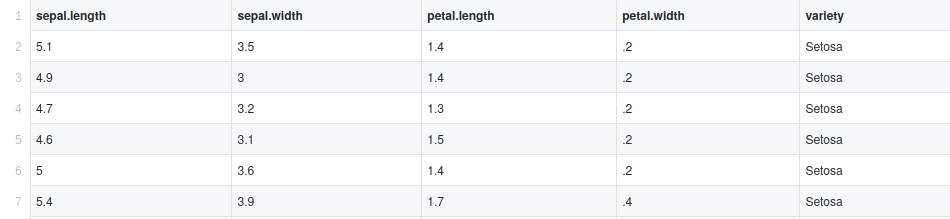
\includegraphics[width = \textwidth]{immagini/Iris}
	\caption{Visualizzazione di un estratto del dataset Iris}
\end{figure}
\section{Incidenti Stradali}
\label{incidentiStradali}
Apprese le basi del Machine Learning ho iniziato a lavorare con il dataset ``Incidenti Stradali'', questo dataset è stato fornito da medici legali e raccoglie, tristemente, i decessi causati appunto da incidenti stradali. Sono state raccolte 131 istanze e ognuna rappresenta una persona deceduta. Il dataset è organizzato in vari livelli di dettaglio. Un primo livello è composto dalle  caratteristiche basilari:
\begin{itemize}
	\item numero del verbale, verrà usato come indice univoco,
	\item data del decesso,
	\item sesso,
	\item anni,
	\item peso,
	\item altezza,
	\item BMI, indice di massa corporea.
\end{itemize}
Successivamente sono descritti i totali delle rotture avvenute nei distretti di:
\begin{itemize}
	\item testa,
	\item torace,
	\item addome,
	\item scheletro.
\end{itemize}
Ogni distretto è poi diviso più nello specifico in singole ossa, ognuna con etichetta che va da 0, nessuna lesione, a 4, lesione massima (cfr. Figura 9).
\begin{figure}[h]
	\centering
	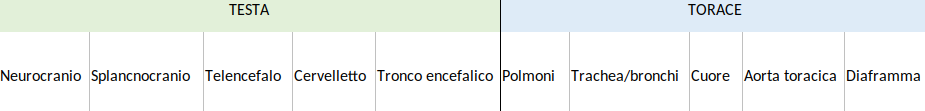
\includegraphics[width = \textwidth]{immagini/testa-torace-dataset}
	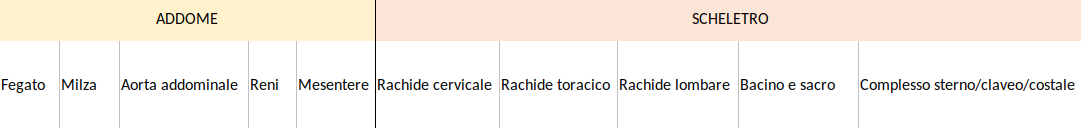
\includegraphics[width = \textwidth]{immagini/addome-scheletro-dataset}
	\caption{Suddivisione caratteristiche dettagliate}
\end{figure}

Il dataset ha inoltre due ulteriori livelli di dettaglio. Esso contiene infatti anche dati più specifici riguardanti la frattura o meno di singole ossa raggruppate in:
\begin{itemize}
	\item cranio,
	\item rachide,
	\item torace - gabbia toracica,
	\item bacino,
	\item arti superiori,
	\item arti inferiori.
\end{itemize}
In ultimo è registrato il mezzo che ha investito la persona. Questo è il label set, la y dei modelli descritti al capitolo precedente. Tutti gli esperimenti effettuati in fase di studio sono incentrati sul cercare di classificare il tipo di mezzo, leggero ovvero auto, etichettato con 0, o pesante, con etichetta 1, che ha investito l'individuo.

Nel mio studio mi sono limitato a considerare le caratteristiche basilari, i totali e quelle riportate in Figura 9.
\section{Riduzione della Dimensionalità}
\label{sec:riduzione}
Nei problemi di classificazione di Machine Learning ci sono spesso molte caratteristiche da tenere in considerazione, basti pensare che il dataset ``Incidenti Stradali'' al completo ha circa 350 caratteristiche. Per dataset con molte dimensioni la riduzione della dimensionalità è un pratica importante svolta prima di applicare algoritmi di Machine Learning per evitare l'effetto chiamato \textit{curse of dimensionality}, ``maledizione della dimensionalità''\cite{shalevshwartz2014understanding}. Il problema sorge nel momento in cui le caratteristiche sono molte e lo spazio aumenta così rapidamente che i dati disponibili diventano radi, sparsi. In ambito statistico questa scarsità è problematica in quanto i dati necessari a supportare il risultato aumentano in modo esponenziale.
Inoltre dati con molte dimensioni possono causare problemi di \textit{overfitting}, ovvero il sistema in qualche modo impara e memorizza il risultato, si adatta (\textit{fitting}) troppo bene (\textit{over}) ai dati di training perdendo di generalità. Il modello sembra perfetto per i dati di training ma quando si prova ad applicarlo ai dati di test si verificano molti errori.
Per questo motivo viene effettuata una riduzione della dimensionalità in modo da eliminare le caratteristiche più irrilevanti e lasciare spazio a quelle rilevanti. 

Gli algoritmi presi in considerazione durante il tirocinio sono PCA e t-SNE, come descritto nei paragrafi che seguono.

\subsection{PCA}
L'idea alla base del pricipal component analysis (PCA), o analisi delle componenti principali, è di ridurre la dimensione di un dataset che contiene un grande numero di caratteristiche correlate, mantenendo il più possibile la varianza presente nel dataset. Quello che si fa è selezionare le componenti principali, che non sono correlate tra di loro e che sono ordinate in modo tale che le prime  mantengano la maggior parte di varianza presente in tutte le caratteristiche iniziali \cite{pca}.

L'idea è di trattare le caratteristiche come una matrice $A$ ottenuta mettendo uno sopra l'altro tutti i vettori nello spazio originale, e trovare gli autovettori per $A A^{T}$ o $A^{T}A$. 

La matrice di questi autovettori può essere vista come una rotazione nello spazio. 
\begin{figure}[h]
\centering
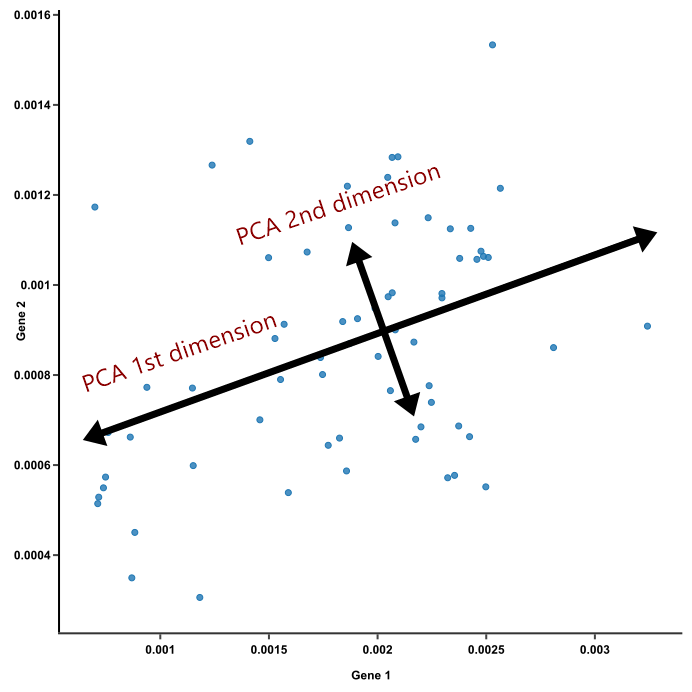
\includegraphics[width = 100mm]{immagini/pca}
\caption{Dimensioni trovate tramite PCA \cite{pcaFigura}}
\end{figure}


Quando si applica questa trasformazione dei dati, l'asse corrispondente all'autovettore principale è quello nel quale i dati sono più sparsi, ovvero l'asse nel quale la varianza dei dati è massimizzata.

Detto in altro modo, i punti possono essere osservati meglio se distesi lungo questo asse, con piccole deviazioni da esso. Allo stesso modo, l'asse corrispondente al secondo autovettore (l'autovettore corrispondente al secondo autovalore più grande) è l'asse lungo il quale la varianza delle distanze dal primo asse è maggiore, e così via fino al numero di dimensioni che si è scelto di mantenere.

Ma come funziona esattamente? 
Per prima cosa si costruisce la matrice dei dati A nel quale ogni colonna corrisponde ad una caratteristica e ogni riga ad una istanza. Successivamente si calcola la media di ogni colonna e la si sottrae ad ogni elemento della matrice, ottenendo così la matrice B.

A questo punto viene calcolata la matrice di covarianza. Ogni valore di covarianza assume un segno: se positivo significa che c'è una correlazione positiva, al contrario, se negativa, c'è una correlazione inversa.

La matrice appena calcolata serve per poter calcolare gli autovalori, operatori che si basano sul fatto che moltiplicando o dividendo un vettore cambia solo la sua lunghezza e non la direzione. Un autovalore $\lambda$ è tale se risolve 
\begin{equation}
Av = \lambda v,
\end{equation}
con $A$ matrice quadrata e $v$ vettore che viene definito autovettore. 

Se per esempio
\begin{equation}
A=\left[\begin{matrix}
1&1\\8&1
\end{matrix}\right]
\text{e } v=\left[\begin{matrix}
1\\2
\end{matrix}\right],
\end{equation}
è facile verificare che $\lambda = 5$ rappresenta un autovalore in quanto risolve l'equazione (9).

Per calcolare gli autovalori di una matrice è possibile risolvere la seguente equazione
\begin{equation}
\det(A - \lambda I) = 0,
\end{equation}
dove $I$ è la matrice identità e $\det$ rappresenta il determinante della matrice.

Avendo trovato il valore di $\lambda$ è possibile calcolare gli autovettori corrispondenti agli autovalori risolvendo l'equazione (9) e trovando $v$:

Gli autovettori trovati formeranno gli assi del nuovo sistema di riferimento di dimensioni più piccole rispetto a quello iniziale. Tuttavia gli autovettori definiscono solo le direzioni degli assi, di conseguenza per decidere quale autovettore vogliamo eliminare per il nostro sottospazio di dimensione inferiore dobbiamo vedere gli autovalori. Quello che faremo sarà eliminare gli autovettori con autovalori più bassi in quanto hanno il minor numero di informazioni sulla distribuzione dei dati al loro interno. Quello che viene fatto è ordinare gli autovalori dal più grande al più piccolo e prendere i primi $k$ autovettori corrispondenti.

In ultimo dobbiamo formare le componenti principali, per farlo calcoliamo:
\begin{equation}
CP = W^{T} \cdot B^{T},
\end{equation}
dove $CP$ è la matrice costituita dalle componenti principali, $W^{T}$ è la matrice formata usando gli autovettori che abbiamo scelto di mantenere precedentementee di cui consideriamo la trasposta, $B^{T}$ è la trasposta della matrice B precedentemente calcolata.
Quello che si ottiene sono i dati originali ma inseriti nello spazio considerando come assi di riferimento gli autovettori calcolati.

Sebbene PCA sia uno degli algoritmi più famosi e usati poiché è veloce, facile da usare e intuitivo ha un problema: è una tecnica lineare, presuppone cioè che i componenti principali siano una combinazione lineare delle caratteristiche originali. Nel caso non sia così non fornirà risultati efficienti. 
Il paragrafo seguente illustra una tecnica non lineare di riduzione della dimensionalità che tende ad adattarsi meglio ai dataset disponibili.
\subsection{t-SNE}
t-SNE, o t-Distributed Stochastic Neighbor Embedding, è una tecnica di riduzione della dimensionalità non lineare \cite{t-SNE}. Utilizza una struttura locale nella quale punti aventi molte dimensioni vengono mappati nello spazio usando un numero inferiore di dimensioni, ciò avviene in modo che punti vicini nello spazio originale vengano trasformati in punti vicini nello spazio con dimensione minore.
 
L'algoritmo prevede tre passi.
\begin{itemize}
	\item Il primo punto calcola una misura di similarità tra i punti nello spazio a molte dimensioni, e centra una distribuzione gaussiana sopra a ogni punto $x_i$. Viene poi calcolato il valore della densità corrispondente per tutti gli altri punti $x_j$. Dopo un processo di normalizzazione, si ottiene un insieme di valori di probabilità $P_{ij}$ che sono che sono proporzionali ai valori di similarità. La distribuzione può essere manipolata usando quella che viene chiamata perplessità, la quale influenza la varianza della distribuzione, ovvero quanto è ampia la curva, che a sua volta influenza  il numero dei vicini di ogni punto. Il normale range della perplessità è tra 5 e 50.
	\item Il secondo punto è simile al primo, ma al posto di una distribuzione gaussiana fa riferimento ad una distribuzione t-Student. Essa ci fornisce un secondo set di probabilità $Q_{ij}$ in uno spazio ridotto. La distribuzione t-Student ha code più lunghe rispetto alla gaussiana(cfr. Figura 11), e questo permette una migliore visualizzazione delle distanze tra i punti.
	
	\begin{figure}[h]
		\centering
		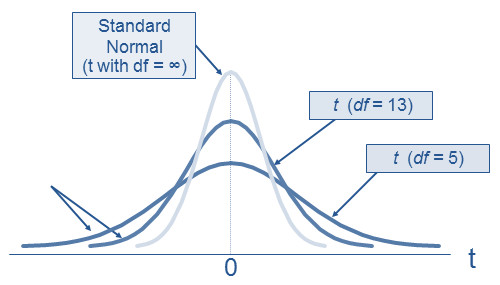
\includegraphics[width = 79mm]{immagini/t-dist1}
		\caption{Grafici della densità delle distribuzioni gaussiana ( curva verde), e t-Student (curva blu). La forma della distribuzione t-Student è data dai gradi di libertà che si riferiscono al numero di osservazioni indipendenti all'interno dei dati}
	\end{figure}
	\item Nel terzo passo si finalizza il calcolo delle probabilità $Q_{ij}$ nello spazio ridotto in modo che riflettano il meglio possibile le probabilità $P_{ij}$ relative allo spazio con più dimensioni. Ciò viene effettuato misurando la differenza tra le due distribuzioni di probabilità usando la divergenza di Kullback-Liebler (KL) che confronta efficacemente valori di $P_{ij}$ e $Q_{ij}$ di grandi dimensioni. Per minimizzare la divergenza di KL tra le due dimensioni viene utilizzata la discesa del gradiente \cite{t-SNE}.
\end{itemize}

Nel \ref{cap3} verranno applicate PCA e t-SNE per cercare di aumentare le prestazioni di classificazione dei modelli usati.



% 
%			CAPITOLO 3: Esperimenti
% 

\chapter{Esperimenti}
\label{cap3}
Durante il tirocinio ho effettuato diversi esperimenti a partire dal dataset descritto al capitolo precedente prendendo in considerazione i diversi livelli di dettaglio \ref{incidentiStradali}, ho usato \emph{python} come linguaggio di programmazione, in particolare il pacchetto \emph{skikit-learn} \cite{scikit-learn} e \emph{Jupyter} come ambiente di lavoro \cite{jupyter}.
In questo capitolo verranno discussi i passaggi necessari per passare dal dataset ad una previsione dell'etichetta corrispondente il più precisa possibile.
\section{Pre Processsing}
\label{preprocessing}
In prima istanza quello che si compie avendo i dati è un processo di pre processing. I dati vengono trasformati o codificati in modo tale che sia più facile per l'algoritmo, che verrà applicato in un secondo momento,  analizzarli e interpretarli.
Consiste in diversi passaggi.
\begin{itemize}
	\item Gestione dei valori null, è necessario gestire i valori nulli prima di fornire i dati all'algoritmo poiché nessun modello è in grado di gestirli autonomamente.
	\item Imputation, ovvero il processo nel quale vengono sostituiti i valori mancanti all'interno del dataset. Per fare questo \emph{sklearn} mette a disposizione la classe \emph{Imputer}.
	\item Standardizzazione, processo di trasformazione dei valori. Questo viene fatto poiché, all'interno del dataset, potrebbero esserci caratteristiche inserite con scale diverse. Prendiamo per esempio un dataset con all'interno due caratteristiche numeriche, ``metratura'' e ``costo'': non sono sulla stessa scala, ``metratura'' si misura in metri quadrati, mentre ``costo'' in euro. 
	\item Gestire le variabili categoriche, variabili che indicano l'appartenenza ad una specifica categoria.
\end{itemize}
Durante il tirocinio come processo di pre-processing ho controllato che il numero del verbale di ogni istanza fosse univoco e che le caratteristiche basilari \ref{incidentiStradali} avessero un valore sensato con quello che stavano rappresentando. Successivamente ho scalato i dati usando tre diversi scaler del pacchetto \emph{preprocessing} di \emph{scikit-learn}:
\begin{itemize}
	\item \emph{StandardScaler},
	\item \emph{MinMaxScaler},
	\item \emph{RobustScaler}.
\end{itemize} 
\subsection{Scalare i dati}
Il processo di scalatura consente di standardizzare i dati. Questa pratica è importante, non solo per riuscire a confrontare caratteristiche con unità di misura diverse, come detto in \ref{preprocessing}, ma anche perché molti algoritmi lavorano meglio con dati impostati in questo modo.  
Analizziamo ora le tre diverse tecniche usate.

\emph{StandardScaler}, standardizza i dati rimuovendo la media $\mu$ e sottraendo la varianza $\sigma$ \cite{scikit-learn}, ovvero:
\begin{equation}
z = \frac{x_i - \mu}{\sigma}.
\end{equation}
Questo viene fatto poiché molti algoritmi assumono che tutte le caratteristiche siano centrate attorno a 0 e abbiano varianza dello stesso ordine. Se una caratteristica presenta una varianza di ordini di grandezza superiore rispetto ad altre, potrebbe influenzare troppo la funzione obiettivo dell'algoritmo usato e rendere lo stimatore incapace di apprendere correttamente da altre caratteristiche \cite{scikit-learn}.

\emph{MinMaxScaler}, ridimensiona singolarmente ogni caratteristica in un determinato intervallo \cite{scikit-learn}, esempio tra 0 e 1. Si applica la seguente formula:
\begin{equation}
X_{norm} = \frac{X - X_{min}}{X_{max} - X_{min}}
\end{equation}
\emph{RobustScaler}, scala le caratteristiche usando statistiche robuste rispetto agli outlier \cite{scikit-learn}. Questo scaler rimuove la mediana e scala i dati in base all'intervallo quantile; è utile perché i valori anomali possono spesso influenzare la media e la  varianza del campione in modo negativo. In tali casi, l'intervallo mediano e quartile danno spesso risultati migliori.

\section{Model Selection}
Il processo di \emph{model selection} è la ricerca del modello più performante dato un set di modelli prodotti da diverse scelte di iperparametri. \cite{Raschka2018ModelEM}.
Durante il tirocinio ho avuto modo di lavorare con i modelli riportati al capitolo \ref{apprendimentoSupervisionato}, ognuno dei quali presenta diversi iperparametri con cui è possibile modificare il comportamento del modello. Vediamo nel dettaglio i vari iperparametri che ho usato durante lo studio sugli incidenti stradali.
 
\subsection{Scelta degli Iperparametri}
\label{iperparametri}
In ogni modello sono presenti diversi iperparametri, ognuno dei quali ha scopi ben precisi. Durante il tirocinio ho usato diversi iperparametri per rendere i modelli più efficienti.
Iniziamo con gli iperparametri di SVC, in particolare di \emph{C}, per un valore di \emph{C} grande è assegnato un grande peso agli errori che risiedono sul margine, quindi diminuisce il bias e aumenta la varianza. Per valori di \emph{C} piccoli invece si ha un bias più grande e una minore varianza. 
Un altro iperparametro di SVC è il \emph{Kernel} che può essere di diversi tipi: \emph{linear}, \emph{polynomial}, \emph{radial basis function}. Associato al kernel di tipo polinomiale c'è inoltre un altro iperparametro chiamato \emph{degree}. Esso consente un limite decisionale più flessibile 
Associato invece ad un kernel di tipo gaussiano c'è \emph{gamma} usato per gestire la classificazione non lineare.
Di seguito viene riportata la griglia con i valori degli iperparametri.

\begin{lstlisting}[frame=single, basicstyle=\footnotesize]
c_space = np.logspace(-4, 3, 10)
gamma_space = np.logspace(-4, 3, 10)

model_selection_grid_SVC = [
{'C': c_space, 'kernel': ['linear'], 'gamma': ['auto']},
{'C': c_space, 'gamma': gamma_space, 'kernel': ['rbf']},
{'C': c_space, 'gamma': ['auto', 'scale'], 'kernel': ['rbf']},
{'C': c_space, 'degree': [2, 3, 5, 9], 'kernel': ['poly'],
'gamma': ['auto']},
]
\end{lstlisting}

Per quanto riguarda Decision Tree abbiamo diversi iperparametri, \emph{criterion}, funzione che viene usata per misurare la qualità della divisione nell'albero e può essere di due tipi: ``gini'' o ``entropy'' \cite{scikit-learn}; \emph{max\_depth}, ovvero la profondità massima dell'albero \cite{scikit-learn}; \emph{max\_features}, il numero di caratteristiche da considerare quando si cerca la migliore divisione \cite{scikit-learn}; \emph{max\_leaf\_nodes}, imposta un limite massimo ai nodi foglia.
\begin{lstlisting}[frame=single, basicstyle=\footnotesize]
model_selection_grid_DT = {'criterion': ['gini', 'entropy'],
'max_leaf_nodes': [None, 2, 5, 10, 50, 100],
'max_features': [None, 'sqrt', 'log2'],
'max_depth': [None, 2, 5, 10]}
\end{lstlisting}

\newpage
In Random Forest troviamo gli stessi iperparametri di Decision Tree con l'aggiunta di \emph{n\_estimators} che rappresenta il numero di  alberi nella foresta.

\begin{lstlisting}[frame=single, basicstyle=\footnotesize]
model_selection_grid_RF = {'n_estimators': [5, 10, 50, 100, 200],
'criterion': ['gini', 'entropy'],
'max_leaf_nodes': [None, 2, 5, 10, 50, 100],
'max_features': [None, 'sqrt', 'log2'],
'max_depth': [None, 2, 5, 10]}
\end{lstlisting}


In Guaussian Naive Bayes e Linear Discriminant Analysis non ho effettuato model selection.

Infine nelle Reti Neurali Multi-Strato ho considerato tre iperparametri: \emph{max\_iter} che specifica il numero massimo di iterazioni; \emph{hidden\_layer\_sizes} rappresenta il numero di neuroni in un livello hidden, esempio: $hidden\_layer\_sizes=[2]$ significa che c'è un livello hidden con due neuroni, mentre $hidden\_layer\_sizes=[4, 4]$ significa che ci sono due livelli hidden ognuno composto da quattro neuroni; infine la funzione di attivazione: \emph{activation} \ref{MLP}.
\begin{lstlisting}[frame=single, basicstyle=\footnotesize]
model_selection_grid_MLP = {'max_iter': [5000],
'hidden_layer_sizes': [[2], [4], [6], [10], [20], [4, 4], [10, 10]],
'activation': ['identity', 'logistic', 'tanh', 'relu']}
\end{lstlisting}


Per effettuare la model selection ho utilizzato \emph{GridSearchCV} fornito dal pacchetto \emph{scikit-learn}, esso effettua una ricerca esaustiva dei valori degli iperparametri del modello, selezionato tramite il parametro \emph{estimator}, specificati all'interno del parametro \emph{param\_grid}. La ricerca degli iperparametri del modello può essere ottimizzata effettuando una cross-validation \ref{cv} sulla griglia degli iperparametri passata in input.

\section{Errore di Generalizzazione}
\label{sec:errore}
L'errore di generalizzazione è una misura di quanto accuratamente un algoritmo è in grado di prevedere i valori delle etichette per nuovi dati.
Il processo che si segue è il seguente: un algoritmo viene ``allenato'' usando degli esempi (\emph{training set}  \ref{ComefunzionailMachineLearning}) di cui è nota l'etichetta che si vuole predire. L'obiettivo è raggiungere uno stato in cui l'algoritmo sia in grado di predire le etichette per altri esempi che non ha avuto in input durante la fase di training. Si dice che così facendo l'algoritmo sarà in grado di \emph{generalizzare}.
L'errore di generalizzazione può essere  minimizzato evitando l'``overfitting'' nell'algoritmo di apprendimento, ovvero il caso in cui l'algoritmo si adatta a caratteristiche che sono specifiche solo del training set e che non hanno riscontro nel resto dei dati. Questo fenomeno si verifica quando i dati di training non sono sufficienti, non sono rappresentativi della realtà oppure quando l'algoritmo prende in considerazione delle caratteristiche del training set irrilevanti con l'etichetta.  Perciò, in presenza di ``overfitting'', le prestazioni sui dati di allenamento aumenteranno, mentre quelle sui dati non visionati saranno peggiori. 

Per prevenire ``overfitting'' viene usata la ``cross-validation'' in modo che l'algoritmo non impari ad adattarsi all'input fornito.
\section{Cross Validation}
\label{cv}
La cross-validation, o k-fold validation, è una tecnica che utilizza parte dei dati disponibili per addestrare il modello e una parte per testarlo \cite{TheElementsofStatisticalLearning}. Viene specificato il numero di ``fold'', ovvero in quante parti dividere il training set. Facciamo un esempio di come funziona, impostiamo a 3 il numero di fold.	Avremo come risultato set divisi come in Figura 12.

\begin{figure}[h]
	\centering
	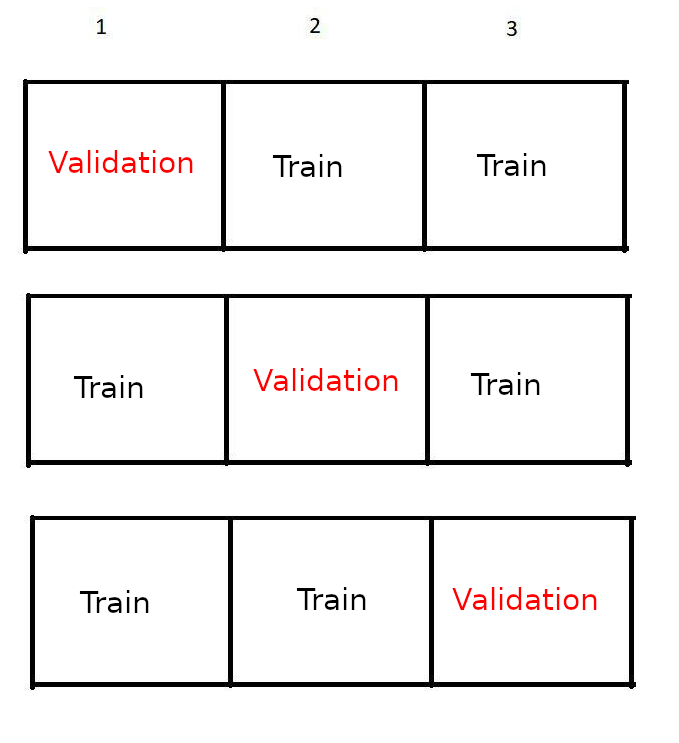
\includegraphics[width = 79mm]{immagini/cross-validation}
	\caption{Cross validation con 3 fold}
\end{figure}
Un set viene assegnato a ``validation test'', mentre i restanti 2 compongono il ``training set''. L'algoritmo viene addestrato usando il training set così composto e testato sul  validation. Questo procedimento viene eseguito per tutte le combinazioni possibili dei set.
Negli esperimenti di paragrafo \ref{sec:risultati} ho usato una cross-validation annidata per stimare l'errore di generalizzazione e fare la model selection usando in entrambi i casi 9 come numero di fold per tutti gli algoritmi nel quale era richiesta una model selection \ref{iperparametri}, quindi per Gaussian Naive Bayes e Linear Discriminant Analysis ho effettuato solo una cross-validation singola per stimare l'errore di generalizzazione.




\section{Risultati Ottenuti}
\label{sec:risultati}
Visualizziamo ora i risultati ottenuti, ogni riga corrisponde ad un esperimento effettuato usando un algoritmo di apprendimento mentre ogni colonna corrisponde al tipo di dataset usato per effettuare l'addestramento. Il dataset ``Details'' ha una dimensione iniziale di 20. Il numero a fianco a ``PCA'' e ``t-SNE'' indica a quante dimensioni si è scesi. Il numero sta ad indicare la percentuale di successo del classificatore, se per esempio troviamo $0.77$ significa che nel $77\%$ dei casi il classificatore ha prodotto l'etichetta corretta.
In azzurro vengono evidenziati gli score massimi del singolo modello mentre in arancione lo score massimo della tabella.

Tabelle generate usando come scaler StandardScaler.
\begin{table}[ht]
	\begin{center}
		\begin{adjustbox}{max width=\textwidth, max totalheight= {3.3cm}}
			\begin{tabular}{lrrrr}
				\toprule
				{} &    Totali &  Totali\_with\_BMI &  Totali\_with\_DATA &  Totali\_with\_DATA\_and\_BMI \\
				\midrule
				SVC &  0.66 &         0.66 &          \cellcolor{orange}0.77 &                  0.73 \\
				DT  &  0.56 &         0.56 &          0.61 &                  0.63 \\
				RF  &  0.64 &         0.63 &          0.57 &                  0.59 \\
				NB  &  0.69 &         0.68 &          0.72 &                  \cellcolor{cyan}0.75 \\
				LD  &  0.71 &         0.68 &          \cellcolor{cyan}0.72 &                  0.72 \\
				MLP &  0.69 &         0.69 &          \cellcolor{cyan}0.74 &                  0.72 \\
				\bottomrule
			\end{tabular}
		\end{adjustbox}
	\end{center}
\end{table}
\begin{table}[h]
	\begin{center}
		\begin{adjustbox}{max width=\textwidth, max totalheight= {4cm}}
			\begin{tabular}{lrrrrrrr}
				\toprule
				{} &   Details &  \thead{Details\\PCA\_5} & \thead{Details\\ PCA\_10} &  \thead{Details\\ PCA\_13} &  \thead{Details\\PCA\_15} &  \thead{Details\\TSNE\_13} &  \thead{Details\\TSNE\_15} \\
				\midrule
				SVC &  0.68 &                  0.63 &                   0.68 &                   0.67 &                   0.71 &                    0.51 &                    0.53 \\
				DT  &  \cellcolor{cyan}0.68 &                  0.60 &                   0.67 &                   0.64 &                   0.57 &                    0.43 &                    0.50 \\
				RF  &  0.67 &                  0.59 &                   0.69 &                   \cellcolor{cyan}0.70 &                   0.63 &                    0.51 &                    0.55 \\
				NB  &  0.63 &                  0.61 &                   0.66 &                   0.67 &                   0.65 &                    0.56 &                    0.57 \\
				LD  &  0.63 &                  0.64 &                   0.60 &                   0.59 &                   0.59 &                    0.48 &                    0.49 \\
				MLP &  0.63 &                  0.62 &                   0.61 &                   0.62 &                   0.65 &                    0.39 &                    0.47 \\
				\bottomrule
			\end{tabular}
		\end{adjustbox}
	\end{center}
\end{table}
\begin{table}[h]
	\begin{center}
		\begin{adjustbox}{max width=\textwidth, max totalheight= {5.5cm}}
			\begin{tabular}{lr}
				\toprule
				{} &  StandardScaler \\
				\midrule
				Totali                     &        0.71 \\
				Totali\_with\_BMI            &        0.69 \\
				Totali\_with\_DATA           &        \cellcolor{orange}0.77 \\
				Totali\_with\_DATA\_and\_BMI   &        0.75 \\
				Details                    &        0.68 \\
				Details\_reduce\_PCA\_5\_dim   &        0.64 \\
				Details\_reduce\_PCA\_10\_dim  &        0.69 \\
				Details\_reduce\_PCA\_13\_dim  &        0.70 \\
				Details\_reduce\_PCA\_15\_dim  &        0.71 \\
				Details\_reduce\_TSNE\_13\_dim &        0.56 \\
				Details\_reduce\_TSNE\_15\_dim &        0.57 \\
				\bottomrule
			\end{tabular}
		\end{adjustbox}
	\end{center}
\end{table}

\newpage

Tabelle generate usando come scaler MinMaxScaler.
\begin{table}[h]
	\begin{center}
		\begin{adjustbox}{max width=\textwidth, max totalheight= {3.3cm}}
			\begin{tabular}{lrrrr}
				\toprule
				{} &    Totali &  Totali\_BMI &  Totali\_DATA &  Totali\_DATA\_and\_BMI \\
				\midrule
				SVC &  0.66 &         0.62 &          0.73 &                  \cellcolor{cyan}0.74 \\
				DT  &  0.61 &         0.55 &          0.65 &                  0.63 \\
				RF  &  0.60 &         0.62 &          0.62 &                  0.61 \\
				NB  &  0.69 &         0.68 &          0.72 &                  \cellcolor{cyan}0.75 \\
				LD  &  0.71 &         0.68 &          \cellcolor{cyan}0.72 &                  0.72\\
				MLP &  0.62 &         0.64 &          0.71 &                  \cellcolor{orange}0.76\\
				\bottomrule
			\end{tabular}
		\end{adjustbox}
	\end{center}
\end{table}

\begin{table}[h]
	\begin{center}
		\begin{adjustbox}{max width=\textwidth, max totalheight= {4cm}}
			\begin{tabular}{lrrrrrrr}
				\toprule
				{} &   Details &  \thead{Details\\PCA\_5} &  \thead{Details\\PCA\_10} &  \thead{Details\\PCA\_13} &  \thead{Details\\PCA\_15} &  \thead{Details\\TSNE\_13} &  \thead{Details\\TSNE\_15} \\
				\midrule
				SVC &  0.74 &                  0.70 &                   0.64 &                   0.67 &                   0.70 &                    0.58 &                    0.42 \\
				DT  &  \cellcolor{cyan}0.70 &                  0.61 &                   0.60 &                   0.56 &                   0.59 &                    0.51 &                    0.56 \\
				RF  &  0.67 &                  0.65 &                   0.66 &                   \cellcolor{cyan}0.71 &                   0.67 &                    0.46 &                    0.52 \\
				NB  &  0.63 &                  0.67 &                   0.65 &                   0.67 &                   0.67 &                    0.57 &                    0.58 \\
				LD  &  0.63 &                  0.65 &                   0.61 &                   0.60 &                   0.62 &                    0.43 &                    0.39 \\
				MLP &  0.65 &                  0.64 &                   0.64 &                   0.60 &                   0.63 &                    0.51 &                    0.43 \\
				\bottomrule
			\end{tabular}
		\end{adjustbox}
	\end{center}
\end{table}

\begin{table}[h]
	\begin{center}
		\begin{adjustbox}{max width=\textwidth, max totalheight={5.5cm}}
			\begin{tabular}{lr}
				\toprule
				{} &  MinMaxScaler \\
				\midrule
				Totali                     &      0.71 \\
				Totali\_with\_BMI            &      0.68 \\
				Totali\_with\_DATA           &      0.73 \\
				Totali\_with\_DATA\_and\_BMI   &      \cellcolor{orange}0.76 \\
				Details                    &      0.74 \\
				Details\_reduce\_PCA\_5\_dim   &      0.70 \\
				Details\_reduce\_PCA\_10\_dim  &      0.66 \\
				Details\_reduce\_PCA\_13\_dim  &      0.71 \\
				Details\_reduce\_PCA\_15\_dim  &      0.70 \\
				Details\_reduce\_TSNE\_13\_dim &      0.58 \\
				Details\_reduce\_TSNE\_15\_dim &      0.58 \\
				\bottomrule
			\end{tabular}
		\end{adjustbox}
	\end{center}
\end{table}

\newpage

Tabelle generate usando come scaler RobustScaler.
\begin{table}[h]
	\begin{center}
		\begin{adjustbox}{max width=\textwidth, max totalheight= {3.3cm}}
			\begin{tabular}{lrrrr}
				\toprule
				{} &    Totali &  Totali\_BMI &  Totali\_DATA &  Totali\_DATA\_and\_BMI \\
				\midrule
				SVC &  0.66 &         0.68 &          \cellcolor{orange}0.77 &                  0.72 \\
				DT  &  0.59 &         0.60 &          0.62 &                  0.65 \\
				RF  &  0.62 &         0.63 &          0.56 &                  0.61 \\
				NB  &  0.69 &         0.68 &          0.72 &                  \cellcolor{cyan}0.75 \\
				LD  &  0.71 &         0.68 &          \cellcolor{cyan}0.72 &                  0.72 \\
				MLP &  0.70 &         0.67 &          \cellcolor{cyan}0.70 &                  0.66 \\
				\bottomrule
			\end{tabular}
		\end{adjustbox}
	\end{center}
\end{table}

\begin{table}[h]
	\begin{center}
		\begin{adjustbox}{max width=\textwidth, max totalheight= {4cm}}
			\begin{tabular}{lrrrrrrr}
				\toprule
				{} &   Details &  \thead{Details\\PCA\_5} &  \thead{Details\\PCA\_10} &  \thead{Details\\PCA\_13} &  \thead{Details\\PCA\_15} &  \thead{Details\\TSNE\_13} &  \thead{Details\\TSNE\_15} \\
				\midrule
				SVC &  0.68 &                  0.63 &                   0.63 &                   0.66 &                   0.66 &                    0.56 &                    0.47 \\
				DT  &  \cellcolor{cyan}0.65 &                  0.63 &                   0.61 &                   0.64 &                   0.63 &                    0.45 &                    0.56 \\
				RF  &  0.65 &                  0.65 &                   0.64 &                   0.64 &                   \cellcolor{cyan}0.66 &                    0.52 &                    0.49 \\
				NB  &  0.63 &                  0.67 &                   0.67 &                   0.67 &                   0.65 &                    0.54 &                    0.56 \\
				LD  &  0.63 &                  0.63 &                   0.60 &                   0.64 &                   0.67 &                    0.43 &                    0.42 \\
				MLP &  0.56 &                  0.63 &                   0.60 &                   0.65 &                   0.60 &                    0.49 &                    0.46 \\
				\bottomrule
			\end{tabular}
		\end{adjustbox}
	\end{center}
\end{table}

\begin{table}[h]
	\begin{center}
		\begin{adjustbox}{max width=\textwidth, max totalheight={5.5cm}}
			\begin{tabular}{lr}
				\toprule
				{} &  RobustScaler \\
				\midrule
				Totali                     &      0.71 \\
				Totali\_with\_BMI            &      0.68 \\
				Totali\_with\_DATA           &      \cellcolor{orange}0.77 \\
				Totali\_with\_DATA\_and\_BMI   &      0.75 \\
				Details                    &      0.68 \\
				Details\_reduce\_PCA\_5\_dim   &      0.67 \\
				Details\_reduce\_PCA\_10\_dim  &      0.67 \\
				Details\_reduce\_PCA\_13\_dim  &      0.67 \\
				Details\_reduce\_PCA\_15\_dim  &      0.67 \\
				Details\_reduce\_TSNE\_13\_dim &      0.56 \\
				Details\_reduce\_TSNE\_15\_dim &      0.56 \\
				\bottomrule
			\end{tabular}
		\end{adjustbox}
	\end{center}
\end{table}



\newpage

Tabelle generate non usando uno scaler e usando direttamente la riduzione di dimensionalità.
\begin{table}[h]
	\begin{center}
		\begin{adjustbox}{max width=\textwidth}
			\begin{tabular}{lrrrrrr}
				\toprule
				{} &  \thead{Details\\PCA\_5} &  \thead{Details\\PCA\_10} &  \thead{Details\\PCA\_13} &  \thead{Details\\PCA\_15} &  \thead{Details\\TSNE\_13} &  \thead{Details\\TSNE\_15} \\
				\midrule
				SVC &                  0.65 &                   0.66 &                   \cellcolor{orange}0.68 &                   0.66 &                    0.57 &                    0.54 \\
				DT  &                  \cellcolor{cyan}0.60 &                   0.55 &                   0.59 &                   0.51 &                    0.50 &                    0.52 \\
				RF  &                  \cellcolor{cyan}0.66 &                   0.64 &                   0.60 &                   0.64 &                    0.53 &                    0.55 \\
				NB  &                  \cellcolor{cyan}0.67 &                   0.64 &                   0.66 &                   0.65 &                    0.52 &                    0.55 \\
				LD  &                  \cellcolor{cyan}0.64 &                   0.62 &                   0.58 &                   0.62 &                    0.47 &                    0.51 \\
				MLP &                  \cellcolor{cyan}0.66 &                   0.65 &                   0.60 &                   0.58 &                    0.43 &                    0.53 \\
				\bottomrule
			\end{tabular}
		\end{adjustbox}
	\end{center}
\end{table}

\begin{table}[h]
	\begin{center}
		\begin{adjustbox}{max width=\textwidth, max totalheight={5.5cm}}
			\begin{tabular}{lr}
				\toprule
				{} &  No\_Scaler \\
				\midrule
				Details\_reduce\_PCA\_5\_dim   &   0.67 \\
				Details\_reduce\_PCA\_10\_dim  &   0.66 \\
				Details\_reduce\_PCA\_13\_dim  &   \cellcolor{orange}0.68 \\
				Details\_reduce\_PCA\_15\_dim  &   0.66 \\
				Details\_reduce\_TSNE\_13\_dim &   0.57 \\
				Details\_reduce\_TSNE\_15\_dim &   0.55 \\
				\bottomrule
			\end{tabular}
		\end{adjustbox}
	\end{center}
\end{table}

\newpage
Tabella riassuntiva generata prendendo le migliori prestazioni usando i dataset e i vari scaler. In arancione troviamo le prestazioni migliori.
\begin{table}[h]
	\begin{center}
		\begin{adjustbox}{max width=\textwidth}
			\begin{tabular}{lrrrr}
				\toprule
				{} &  StandardScaler &  MinMaxScaler &  RobustScaler &  No\_Scaler \\
				\midrule
				Totali                     &        0.71 &      0.71 &      0.71 &        NaN \\
				Totali\_with\_BMI            &        0.69 &      0.68 &      0.68 &        NaN \\
				Totali\_with\_DATA           &        \cellcolor{orange}0.77 &      0.73 &      \cellcolor{orange}0.77 &        NaN \\
				Totali\_with\_DATA\_and\_BMI   &        0.75 &      0.76 &      0.75 &        NaN \\
				Details                    &        0.68 &      0.74 &      0.68 &        NaN \\
				Details\_reduce\_PCA\_5\_dim   &        0.64 &      0.70 &      0.67 &   0.67 \\
				Details\_reduce\_PCA\_10\_dim  &        0.69 &      0.66 &      0.67 &   0.66 \\
				Details\_reduce\_PCA\_13\_dim  &        0.70 &      0.71 &      0.67 &   0.68 \\
				Details\_reduce\_PCA\_15\_dim  &        0.71 &      0.70 &      0.67 &   0.66 \\
				Details\_reduce\_TSNE\_13\_dim &        0.56 &      0.58 &      0.56 &   0.57 \\
				Details\_reduce\_TSNE\_15\_dim &        0.57 &      0.58 &      0.56 &   0.55 \\
				\bottomrule
			\end{tabular}
		\end{adjustbox}
	\end{center}
\end{table}




		

\section{Analisi dei  Risultati}
Osservando i risultati ci si accorge di come non ci sia uno scaler che si comporta meglio in maniera assoluta. 
La riduzione della dimensionalità, eseguita con PCA e t-SNE non comporta un aumento delle prestazioni, anzi molto spesso genera un risultato meno prestante rispetto al dataset di partenza ``Details''. Si può inoltre notare che, all'interno delle tabelle, non sono presenti esperimenti effettuati usando ``Details'' con riduzione della dimensionalità a 5 e 10 dimensioni tramite t-SNE. Questo perché durante l'addestramento t-SNE non è riuscito a convergere e quindi l'addestramento non è riuscito.
In ogni caso i risultati ottenuti usando t-SNE non superano mai lo $0.58$. Si comporta meglio PCA generando score che hanno come range $0.64$ - $0.71$.
I risultati migliori però li abbiamo considerando i ``Totali'', in particolare i dataset ``Totali\_with\_DATA'' e ``Totali\_with\_DATA\_and\_BMI'' sono quelli che generano gli score migliori. In particolare lo score in assoluto più alto è generato usando ``Totali\_with\_DATA'' usando come scaler StandardScaler e RobustScaler con $0.77$.




% 
%			CAPITOLO 4: Conclusioni e sviluppi futuri
% 
\chapter{Conclusioni}

Nelle conclusioni si tirano le somme di quanto realizzato, facendo un riassunto stringato del lavoro svolto. In particolare vanno dichiarati punti di forza e criticità della ricerca effettuata, nonché quali aspetti dello stato dell'arte siano stati superati dal lavoro in oggetto.

%
%			BIBLIOGRAFIA
%

\bibliographystyle{unsrt}
\bibliography{bibliografia}
\addcontentsline{toc}{chapter}{Bibliografia}

\end{document}


 